\documentclass{article}
    \title{\textbf{5. MĚŘICÍ ZESILOVAČE}}
    \author{Tomáš Kysela}
    \date{28/2/2022}

    \addtolength{\topmargin}{-3cm}
    \addtolength{\textheight}{3cm}

\usepackage[czech]{babel}
\usepackage{graphicx}
\usepackage{circuitikz}
\usepackage{amsmath}
\usepackage{subcaption}
\usepackage{pgfplots}
\usepackage{float}
\usepackage{siunitx}
\sisetup{detect-all}

\makeatletter
\providecommand\add@text{}
\newcommand\tagaddtext[1]{%
    \gdef\add@text{#1\gdef\add@text{}}}%
\renewcommand\tagform@[1]{%
    \maketag@@@{\llap{\add@text\quad}(\ignorespaces#1\unskip\@@italiccorr)}%
}
\makeatother


\begin{document}

\maketitle

\section{Úkol měření}
\begin{enumerate}
	\item Změřte napětí termočlánku předloženým číslicovým voltmetrem pro jednu polohu přepínače termostatu.
	\item S použitím operačního zesilovače OP 07 navrhněte zapojení:
	\begin{enumerate}
		\item invertujícího zesilovače napětí se zesílením -100 a vstupním odporem 1 \si{\kilo\ohm}
		\item neinvertujícího zesilovače napětí se zesílením 100 a vstupním odporem 100 \si{\kilo\ohm}	\end{enumerate}
	\item Invertující zesilovač napětí použijte pro zesílení napětí termočlánku, napětí na výstupu zesilovače změřte stejným číslicovým voltmetrem a pro stejnou  polohu  přepínače termostatu jako v bodě 1. Korigujte chybu metody způsobenou konečným vstupním odporem zesilovače.
	\item Určete rozšířenou nejistotu měření napětí termočlánku (koeficient rozšíření kr = 2) jak pro přímé měření číslicovým voltmetrem, tak pro měření napětí termočlánku  po	zesílení invertujícím zesilovačem napětí.
	
	Při určení celkové nejistoty typu  B  měření  zesíleného  napětí termočlánku uvažujte i nejistotu způsobenou vstupní napěťovou nesymetrií operačního zesilovače. Nejistoty způsobené vstupními klidovými proudy zesilovače zanedbejte.
	\item Pro polohu přepínače  termostatu použitou při měřeních dle bodů 1 a 3 určete teplotu teplého konce termočlánku (teplotu měřenou termočlánkem), je-li konstanta použitého termočlánku K = 54 \si{\micro\volt\per\degreeCelsius}. Předpokládejte, že teplota srovnávacích (studených) konců termočlánku je 20 °C (teplota laboratoře).
	\item Ověřte, zda je skutečná vstupní napěťová nesymetrie použitého operačního zesilovače menší než maximální (případně typická) hodnota udaná výrobcem.
\end{enumerate}
\textit{Poznámky k měření:}
\begin{enumerate}
	\item Měřte  až  po  dosažení  tepelného  ustálení  obvodu,  které  indikuje  zánik  monotónních  změn údaje číslicového voltmetru (ustálení údaje až na případný vliv šumu).
	\item Tolerance použitých rezistorů a vnitřní odpor termočlánku jsou uvedeny na přípravcích.
	\item Operační zesilovač umožňuje kompenzaci vstupní napěťové nesymetrie a vstupních klidových proudů zesilovače pomocí nastavitelného rezistoru (odporového trimru). V praxi se ale tato kompenzace zpravidla nepoužívá a ani v přípravku není zapojena.
\end{enumerate}

\section{Schéma zapojení}
\begin{figure}[H]
	\centering
	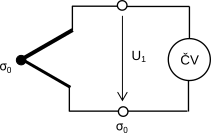
\includegraphics{scheme1}
	\caption{Přímé měření napětí termočlánku číslicovým voltmetrem}
	\label{fig:scheme1}
\end{figure}
\begin{figure}[H]
	\centering
	\begin{subfigure}{0.5\textwidth}
		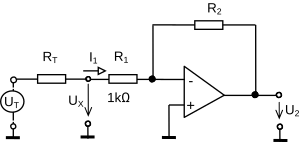
\includegraphics[scale=0.7]{scheme2}
		\caption{Invertující}
		\label{fig:scheme2}
	\end{subfigure}
	\begin{subfigure}{0.45\textwidth}
		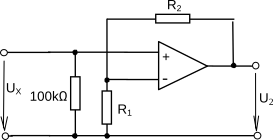
\includegraphics[scale=0.7]{scheme3}
		\caption{Neinvertující}
		\label{fig:scheme3}
	\end{subfigure}
	\caption{zesilovač}
\end{figure}
\begin{table}[h]
	\begin{tabular}{|l||l|l|l|l|l|}
		\hline
		 \textbf{Vlastnost} & \textbf{ICL 7650} & \textbf{741}& \textbf{LT 1097} & \textbf{OP 07}     & \textbf{LM 155} \\ \hline \hline
		napěťový offset  typ./max. (\si{\micro\volt}) & 0.7      & 1500/5000 & 10/60   & 60/150    & 1000   \\ \hline
		jeho teplotní drift (\si{\micro\volt\per\degreeCelsius})     & 0.02     & 10        & 0.3     & 0.5       & 5      \\ \hline
		jeho teplotní drift (\si{\micro\volt\per\degreeCelsius})     & 5        & 50000     & 350     & 1800/7000 & 50     \\ \hline
		CMRR (\si{\decibel})                       & 120      & 90        & 130     & 110       & 100    \\ \hline
		rychlost přeběhu (\si{\volt\per\second})         & 2.5      & 0.5       & 0.2     & 0.3       & 5      \\ \hline
	\end{tabular}
\end{table}
\section{Soupis použitých přístrojů}



\section{Teoretický základ}


\end{document}
